\documentclass{beamer}
\usepackage[utf8]{inputenc}

\usetheme{Madrid}
\usecolortheme{default}
\usepackage{extarrows}
\usepackage{amsmath}
\usepackage{extarrows}
\usepackage{amssymb,amsfonts,amsthm}
\usepackage{txfonts}
\usepackage{tkz-euclide}
\usepackage{listings}
\usepackage{adjustbox}
\usepackage{array}
\usepackage{tabularx}
\usepackage{gvv}
\usepackage{lmodern}
\usepackage{circuitikz}
\usepackage{tikz}
\usepackage{graphicx}
\usepackage{amsmath} 

\setbeamertemplate{page number in head/foot}[totalframenumber]

\usepackage{tcolorbox}
\tcbuselibrary{minted,breakable,xparse,skins}

\definecolor{bg}{gray}{0.95}
\DeclareTCBListing{mintedbox}{O{}m!O{}}{%
  breakable=true,
  listing engine=minted,
  listing only,
  minted language=#2,
  minted style=default,
  minted options={%
    linenos,
    gobble=0,
    breaklines=true,
    breakafter=,,
    fontsize=\small,
    numbersep=8pt,
    #1},
  boxsep=0pt,
  left skip=0pt,
  right skip=0pt,
  left=25pt,
  right=0pt,
  top=3pt,
  bottom=3pt,
  arc=5pt,
  leftrule=0pt,
  rightrule=0pt,
  bottomrule=2pt,
  toprule=2pt,
  colback=bg,
  colframe=orange!70,
  enhanced,
  overlay={%
    \begin{tcbclipinterior}
    \fill[orange!20!white] (frame.south west) rectangle ([xshift=20pt]frame.north west);
    \end{tcbclipinterior}},
  #3,
}
\lstset{
    language=C,
    basicstyle=\ttfamily\small,
    keywordstyle=\color{blue},
    stringstyle=\color{orange},
    commentstyle=\color{green!60!black},
    numbers=left,
    numberstyle=\tiny\color{gray},
    breaklines=true,
    showstringspaces=false,
}
\title %optional
{5.8.30}


\author 
{Kartik Lahoti - EE25BTECH11032}

\begin{document}


\frame{\titlepage}
\begin{frame}{Question}
Rambha travels $300\,km$ to her home partly by train and partly by bus. She takes $4$ hours 
if she travels $60\,km$ by train and the remaining by bus. If she travels $100\,km$ by train and the remaining by bus, she takes $10$ minutes longer. Find the speed of the train and the bus seperately.
\end{frame}

\begin{frame}{Given}

\begin{table}[H]
    \centering
    \begin{tabular}{|c|c|}
\hline
\textbf{Name} & \textbf{Value} \\
\hline
Circle & $\vec{x}^\top\vec{x} - a^2 = 0$ \\
\hline
Line & $\vec{x} = \myvec{\tfrac{a}{\sqrt{2}} \\ 0} + \kappa\myvec{0 \\ 1}$ \\
\hline
\end{tabular}

    \caption{5.8.30}
    \label{table_1}
\end{table}

\end{frame}

\begin{frame}{Theoretical Solution}
Let the equations be,

\begin{align}
    \vec{n_1}^{\top}\vec{X} = c_1 \\ 
    \vec{n_2}^{\top}\vec{X} = c_2 
\end{align}

Since $\vec{P}$ satisfies both the lines, 

\begin{align}
    \vec{n_1}^{\top}\vec{P} = c_1 \\ 
    \vec{n_2}^{\top}\vec{P} = c_2 
\end{align}
\end{frame}

\begin{frame}{Theoretical Solution}
Solving for $\vec{P}$

\begin{align}
    \augvec{2}{1}{60 & 240 & 4\\100 & 200 & \frac{25}{6}}\xleftrightarrow[]{R_1\rightarrow \frac{R_1}{60}}\augvec{2}{1}{1 & 4 & \frac{1}{15}\\100 & 200 & \frac{25}{6}}
\end{align}
\begin{align}
    \augvec{2}{1}{1 & 4 & \frac{1}{15}\\100 & 200 & \frac{25}{6}}\xleftrightarrow[]{R_2\rightarrow \frac{R_2}{100}}\augvec{2}{1}{1 & 4 & \frac{1}{15}\\1 & 2 & \frac{1}{24}}
\end{align}
\end{frame}

\begin{frame}{Theoretical Solution}

\begin{align}
    \augvec{2}{1}{1 & 4 & \frac{1}{15}\\1 & 2 & \frac{1}{24}}\xleftrightarrow[]{R_2\rightarrow R_2 - R_1}\augvec{2}{1}{1 & 4 & \frac{1}{15}\\0 & -2 & \frac{-1}{40}}
\end{align}

\begin{align}
    \augvec{2}{1}{1 & 4 & \frac{1}{15}\\0 & -2 & \frac{-1}{40}} \xleftrightarrow[]{R_2\rightarrow \frac{R_2}{-2} }\augvec{2}{1}{1 & 4 & \frac{1}{15}\\0 & 1 & \frac{1}{80}}
\end{align}
\end{frame}
\begin{frame}{Theoretical Solution}
\begin{align}
    \augvec{2}{1}{1 & 4 & \frac{1}{15}\\0 & 1 & \frac{1}{80}} \xleftrightarrow[]{R_1\rightarrow R_1 - 4R_2 }\augvec{2}{1}{1 & 0 & \frac{1}{60}\\0 & 1 & \frac{1}{80}}
\end{align}

\begin{align}
    \therefore \vec{P} = \myvec{\frac{1}{60} \\ \frac{1}{80}}
\end{align}
\end{frame}

\begin{frame}{Theoretical Solution}
Since $\vec{P}$ is the reciprocal of the speeds 

The speed of train is $60\,km/h$ and bus is $80\,km/h$
\end{frame}

\begin{frame}[fragile]
    \frametitle{C Code - To find inverse of a Matrix }
    \begin{lstlisting}
#include <stdio.h>
#include <math.h>
void row_mal(double X[][3] , double k , int n , int m)
{
    for(int i = 0 ; i< 3 ; i++)
    {
        X[n][i] = X[n][i] - k * X[m][i];
    }
}

void row_div(double X[][3] , double k , int n )
{
    for(int i = 0 ; i< 3 ; i++)
    {
        X[n][i] /= k ;
    }
}
    \end{lstlisting}
\end{frame}


\begin{frame}[fragile]
    \frametitle{C Code  }
    \begin{lstlisting}
void augment(double *A , double *B , double *C)
{
    double X[2][3];
    for(int i = 0; i< 2 ; i++){
        X[i][0] = A[i];
        X[i][1] = B[i];
        X[i][2] = C[i];
    }
    if(X[0][0] != 0 ){
        row_div(X,X[0][0],0);
        if(X[1][0] != 0)
            row_mal(X,X[1][0],1,0);
    }
    else{
        row_mal(X,-1,0,1);
        row_div(X,X[0][0],0);
        if(X[1][0] != 0)
            row_mal(X,X[1][0],1,0);
    }

\end{lstlisting}
\end{frame}

\begin{frame}[fragile]
    \frametitle{C Code  }
    \begin{lstlisting}    
    if(X[1][1] != 0 ){
        row_div(X,X[1][1],1);
        if(X[0][1] != 0)
            row_mal(X,X[0][1],0,1);
    }
    else{
        row_mal(X,-1,1,0);
        row_div(X,X[1][1],1);
        if(X[0][1] != 0)  
            row_mal(X,X[0][1],0,1);
    }
    for(int i = 0 ; i< 2 ; i++){
        C[i] = 1 / X[i][2] ;
        for(int j = 0; j < 3; j++)
            printf("%.3f ",X[i][j]);
        printf("\n");
    }           
}

\end{lstlisting}
\end{frame}

\begin{frame}[fragile]
    \frametitle{C Code - To generate Line  }
    \begin{lstlisting}    
void linegen(double *XY, double *A , double *B , int n , int m )
{
    double temp[m] ; 
    for (int i = 0 ; i < m ; i++)
    {
        temp [ i ] = (B[i]- A[i]) /(double) n ; 
    }
    for (int i = 0 ; i < n ; i++ )
        for (int j = 0 ; j < m ; j++)
            XY[j*n + i ] = A[j] + temp[j] * i ; 
           
}
\end{lstlisting}
\end{frame}

\begin{frame}[fragile]
    \frametitle{Python Code}
    \begin{lstlisting}
import ctypes as ct
import numpy as np
import matplotlib.pyplot as plt

handc1 = ct.CDLL("./func.so")

handc1.augment.argtypes = [
    ct.POINTER(ct.c_double),
    ct.POINTER(ct.c_double),
    ct.POINTER(ct.c_double)
]
handc1.augment.restype = None
A = np.array([60,100] , dtype = np.float64).reshape(-1,1)
B = np.array([240,200] , dtype = np.float64).reshape(-1,1)
C = np.array([4,25/6], dtype = np.float64).reshape(-1,1)

\end{lstlisting}
\end{frame}

\begin{frame}[fragile]
    \frametitle{Python Code}
    \begin{lstlisting}
handc1.augment(
    A.ctypes.data_as(ct.POINTER(ct.c_double)),
    B.ctypes.data_as(ct.POINTER(ct.c_double)),
    C.ctypes.data_as(ct.POINTER(ct.c_double))
)

print("Speed of Train : ",C[0]);
print("Speed of Bus : ",C[1]);

\end{lstlisting}
\end{frame}

\begin{frame}[fragile]
    \frametitle{Python Code}
    \begin{lstlisting}
def line(P: np.ndarray , Q: np.ndarray, str1 , str2):
    handc2 = ct.CDLL("./line_gen.so")

    handc2.linegen.argtypes = [
        ct.POINTER(ct.c_double),
        ct.POINTER(ct.c_double),
        ct.POINTER(ct.c_double),
        ct.c_int , ct.c_int
    ]

    handc2.linegen.restype = None

\end{lstlisting}
\end{frame}
\begin{frame}[fragile]
    \frametitle{Python Code}
    \begin{lstlisting}
n = 200
    XY = np.zeros((2,n),dtype=np.float64)

    handc2.linegen (
        XY.ctypes.data_as(ct.POINTER(ct.c_double)),
        P.ctypes.data_as(ct.POINTER(ct.c_double)),
        Q.ctypes.data_as(ct.POINTER(ct.c_double)),
        n,2
    )
    plt.plot(XY[0,:],XY[1,:], str1 , label = str2 )

\end{lstlisting}
\end{frame}
\begin{frame}[fragile]
    \frametitle{Python Code}
    \begin{lstlisting}
plt.figure()
M = np.array([61/15,-1],dtype=np.float64).reshape(-1,1)
N = np.array([-10,151/60],dtype=np.float64).reshape(-1,1)
line(M,N,"g-","Line 1 ")
M = np.array([2+1/24 , -1],dtype=np.float64).reshape(-1,1)
N = np.array([-10,5+1/48],dtype=np.float64).reshape(-1,1)
line(M,N,"r-","Line 2")
plt.scatter(1/np.squeeze(C[0]),1/np.squeeze(C[1]))
plt.annotate(f"P\n(1/{np.squeeze(C[0]):.0f},1/{np.squeeze(C[1]):.0f})",(1/np.squeeze(C[0]),1/np.squeeze(C[1])),textcoords = "offset points" ,xytext = (0,-25),ha = "center")

\end{lstlisting}
\end{frame}
\begin{frame}[fragile]
    \frametitle{Python Code}
    \begin{lstlisting}
plt.xlim([-1/2,1/2])
plt.ylim([-1/2,1/2])
plt.xlabel("$x$")
plt.ylabel("$y$")
plt.grid()
plt.legend(loc="best")
plt.title("5.8.30")

plt.savefig("../figs/Inter1.png")
plt.show()
#plt.savefig('../figs/Inter1.png')
#subprocess.run(shlex.split("termux-open ../figs/Inter1.png"))

\end{lstlisting}
\end{frame}
\begin{frame}[fragile]
    \frametitle{Python Code - 2 }
    \begin{lstlisting}
import math
import sys 
sys.path.insert(0, '/home/kartik-lahoti/matgeo/codes/CoordGeo')
import numpy as np
import numpy.linalg as LA
import matplotlib.pyplot as plt

from line.funcs import *
A = np.array([[60,240],[100,200]] , dtype = np.float64)
C = np.array([4,25/6], dtype = np.float64).reshape(-1,1)
sol = LA.solve(A,C)

print("Speed of Train = " , 1/sol[0])
print("Speed of Bus = " , 1/sol[1])

\end{lstlisting}
\end{frame}

\begin{frame}[fragile]
    \frametitle{Python Code - 2 }
    \begin{lstlisting}
def plot_it(P,Q,str1,str2):
    x_l = line_gen_num(P,Q,20)
    plt.plot(x_l[0,:],x_l[1,:] , str1 , label =  str2)

plt.figure()
M = np.array([61/15,-1],dtype=np.float64).reshape(-1,1)
N = np.array([-10,151/60],dtype=np.float64).reshape(-1,1)
plot_it(M,N,"g-","Line 1 ")
M = np.array([2+1/24 , -1],dtype=np.float64).reshape(-1,1)
N = np.array([-10,5+1/48],dtype=np.float64).reshape(-1,1)
plot_it(M,N,"r-","Line 2")

\end{lstlisting}
\end{frame}
\begin{frame}[fragile]
    \frametitle{Python Code - 2 }
    \begin{lstlisting}
plt.scatter(np.squeeze(sol[0]),np.squeeze(sol[1]))
plt.annotate(f"P\n(1/{1/np.squeeze(sol[0]):.0f},1/{1/np.squeeze(sol[1]):.0f})",(np.squeeze(sol[0]),np.squeeze(sol[1])),textcoords = "offset points" ,xytext = (0,-25),ha = "center")

plt.xlim([-1/2,1/2])
plt.ylim([-1/2,1/2])

plt.xlabel("$x$")
plt.ylabel("$y$")
plt.grid()

\end{lstlisting}
\end{frame}
\begin{frame}[fragile]
    \frametitle{Python Code - 2 }
    \begin{lstlisting}
plt.legend(loc="best")

plt.title("5.8.30")

plt.savefig("../figs/Inter2.png")
plt.show()

#plt.savefig('../figs/Inter2.png')
#subprocess.run(shlex.split("termux-open ../figs/Inter2.png"))

\end{lstlisting}
\end{frame}
\begin{frame}{Plot}
    \centering
    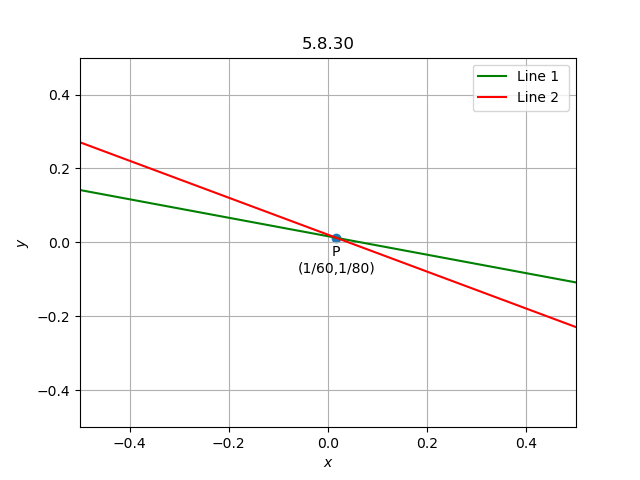
\includegraphics[width=\columnwidth, height=0.8\textheight, keepaspectratio]{../figs/Inter1.png}   
\end{frame}

\end{document}
